% !TeX program = xelatex
% !TeX encoding = UTF-8
% 在 reports/final 目录下编译：xelatex T1_最终报告.tex（两遍）。字体随仓库附带。
% 【待补】标记的内容需要组内补实验或确认后填写，提交前全文搜索“待补”清零。
\documentclass[UTF8,zihao=-4,fontset=none,a4paper]{ctexart}
\setCJKmainfont[Path=../../t1_proposal_latex/fonts/,BoldFont=NotoSerifSC-Bold.otf]{NotoSerifSC-Regular.otf}
\setCJKsansfont[Path=../../t1_proposal_latex/fonts/,BoldFont=NotoSerifSC-Bold.otf]{NotoSerifSC-Regular.otf}
\setCJKmonofont[Path=../../t1_proposal_latex/fonts/,BoldFont=NotoSerifSC-Bold.otf]{NotoSerifSC-Regular.otf}
\usepackage[left=2.2cm,right=2.2cm,top=2.2cm,bottom=2.2cm]{geometry}
\usepackage{amsmath,amssymb,bm}
\usepackage{booktabs,tabularx,array,multirow}
\usepackage{graphicx}
\usepackage{enumitem}
\usepackage{xcolor}
\usepackage{fancyhdr}
\usepackage{caption}
\usepackage[colorlinks=true,linkcolor=black,citecolor=black,urlcolor=teal]{hyperref}
\usepackage{microtype}
\usepackage{xurl}
\definecolor{teal}{HTML}{00766D}
\definecolor{todo}{HTML}{B4361E}
\newcommand{\pending}[1]{{\color{todo}【待补：#1】}}
\newcommand{\tbd}{{\color{todo}【待补】}}
\hypersetup{pdftitle={胚胎心脏发育的时间外推：细胞组成与表达变化的统计分析},
  pdfauthor={高景行, 王恒毅, 李凯瑞, 崔帅达},
  pdfsubject={2026 秋季《统计学习》期末报告，Virtual Embryo Challenge T1}}
\linespread{1.18}
\setlength{\parskip}{3pt}
\setlength{\headheight}{15pt}
\setlist{nosep,leftmargin=2em}
\captionsetup{font=small,labelfont=bf,labelsep=quad}
\ctexset{section={format=\large\bfseries,beforeskip=10pt,afterskip=5pt},
  subsection={format=\normalsize\bfseries,beforeskip=6pt,afterskip=3pt}}
\pagestyle{fancy}
\fancyhf{}
\fancyhead[L]{\small 2026 秋季《统计学习》期末报告}
\fancyhead[R]{\small Virtual Embryo Challenge T1}
\fancyfoot[C]{\small\thepage}
\renewcommand{\headrulewidth}{0.3pt}
\newcolumntype{Y}{>{\raggedright\arraybackslash}X}
\newcommand{\smalltable}{\small\renewcommand{\arraystretch}{1.2}}

\begin{document}
\begin{center}
{\zihao{3}\bfseries 胚胎心脏发育的时间外推：细胞组成与表达变化的统计分析\par}
\vspace{4pt}
{\normalsize NeurIPS 2026 Virtual Embryo Challenge，任务一（Temporal）\par}
\vspace{4pt}
{\small 高景行\quad 王恒毅\quad 李凯瑞\quad 崔帅达\par}
\vspace{2pt}
{\small 代码：\url{https://github.com/ManchesterCityWhy/Statistical_Learning_Term_Project}\par}
\end{center}

\begin{quote}\small
\textbf{摘要}\quad 任务一要求根据较早发育阶段的单细胞 RNA 数据，预测小鼠心脏区域在未来阶段的细胞表达分布。我们以 E8.5、E9.5 和公开的 bulk RNA-seq 为输入，在 E10.5 上做开发验证，最终从 E10.5 预测隐藏的 E12.5。按开题设想实现的全基因外推、PCA 外推和官方的类型平移，在单次抽样的比较中都没有超过“复制最近阶段”基线（46.2--49.2 分，基线 50 分）。按指标拆分后，拖分的是差异基因恢复（DES）和基因共变（CSS）：用两阶段均值差排出的差异基因不如“按表达量排序”，加性平移又把大量零表达变成小正值。随后我们用外部 bulk 数据估计基因变化趋势，并用带岭惩罚的非负最小二乘反卷积调整细胞类型比例，在本地选模集上得到 60.50 分；固定模型后，在复核集和三组审计集上分别得到 59.79 和 59.27--60.48 分。增益主要来自变化方向（DCS）和细胞状态分布（MMD）两项，DES 几乎没有提高。所有模型在复核集上都比选模集低约 0.7 分，未参与挑选的旧方法也一样，所以这次回落来自复核集本身，看不出额外的选模偏差。模型给出的细胞类型权重与 E9.5 的实际组成相差很大，不能当作生物学比例来解读。两次官方 E12.5 提交分别得 70.62 和 73.37 分，都低于公开榜上方法名写着用真实细胞的条目（77.07--80.57 分）；第二次提交改动了细胞组成和表达，我们把它作为一个反面案例分析（第~\ref{sec:negative}~节）。
\end{quote}

\section{研究问题与背景}

胚胎发育伴随细胞分化、群体比例的改变和基因表达模式的改变。单细胞 RNA 测序（scRNA-seq）能在每个时间点观测成千上万个细胞，但测序会破坏细胞，同一个细胞无法在两个时间点重复测量，所以相邻阶段之间只有群体层面的对应关系。已有工作用最优传输在这样的时间快照之间推断细胞的演化\cite{schiebinger}。如果能根据已观测的阶段预测下一阶段的细胞群体，就可以在计算上预先评估发育进程，减少需要实际采样的时间点。

Virtual Embryo Challenge 任务一把这个问题具体化为分布预测：给定较早阶段的细胞表达矩阵，提交一组预测细胞的表达向量，由主办方与隐藏阶段的真实细胞比较\cite{task}。被比较的是两组细胞的分布，不要求预测与真实细胞一一对应，也不要求细胞数相同。

我们关心的问题是：\textbf{在只有两个早期观测阶段的条件下，未来阶段细胞群体的变化，有多少可以由细胞组成的改变解释，又有多少来自细胞内部的表达变化？简单、可解释的统计模型能把预测改进到什么程度，又在哪里失败？} 围绕这个问题，我们比较了三类模型：直接平移表达均值的外推模型，引入外部 bulk 趋势的表达迁移模型，以及调整细胞类型比例的组成模型。对每类模型，我们都按评价指标拆分得分，分析增益和退化的来源。

\section{数据与使用范围}

\subsection{竞赛数据}

任务一的数据是以心脏为中心的小鼠胚胎解剖样本，每个阶段一个 AnnData 文件，\texttt{.X} 为 $\log(1+x)$ 归一化后的表达值，共 32,285 个基因，训练阶段带细胞类型注释\cite{data}。各阶段的角色见表~\ref{tab:data}。决赛阶段开始后，团队可以申请下载 E10.5 的真实表达，申请后不能再向验证榜提交；E12.5 的真值始终不公开。

\begin{table}[h]
\centering\smalltable
\caption{任务一各阶段在本项目中的用途（E10.5、E12.5 的细胞数官方页面未列出）}\label{tab:data}
\begin{tabularx}{\linewidth}{@{}p{1.4cm}p{2.0cm}p{2.0cm}Y@{}}
\toprule
阶段 & 细胞数 & 官方角色 & 本项目用途\\
\midrule
E8.5 & 16,787 & 训练 & 均值平移类方法的较早参照\\
E9.5 & 17,057 & 训练 & 开发验证的源细胞和评分参考\\
E10.5 & -- & 验证 & 开发验证与选模；最终预测的源阶段\\
E12.5 & -- & 隐藏测试 & 只由官方评分，不接触真值\\
\bottomrule
\end{tabularx}
\end{table}

数据有两个特点会直接影响建模。第一，解剖范围随阶段变化：神经管细胞在 E8.5 占 4.6\%，在 E9.5 为 0\%，轴旁中胚层和胚外中胚层也有类似情况\cite{data}。所以目标阶段的细胞组成同时反映发育和取样，模型无法区分这两者。第二，各阶段的注释词表没有统一：E8.5 和 E9.5 分别有 18 和 21 个标签，完全同名的只有 11 个；E9.5 与 E10.5 之间是 23 个类型中有 13 个同名，两次都大约只有一半细胞在前一阶段有同名类型\cite{task}。E9.5 的 Endocardium 在之后的阶段拆成了 Endocardium-1 和 Endocardium-2\cite{data}。我们在中期报告中算过 E8.5 与 E9.5 细胞类型比例的总变差距离：按两阶段标签的并集算为 0.595，只保留同名标签并重新归一化后为 0.297。这个差距既来自词表不一致，也来自解剖范围的变化，因此按名称匹配细胞类型只能作为粗略的对照。

\subsection{外部数据与合规}

竞赛规则允许任务一使用公开外部数据，但要求在提交时披露；规则同时规定，晚于 E9.5、不晚于 E13.5 的外部数据不能用，E9.5 本身和 E13.5 以后的数据可以用\cite{rules}。第一到三轮的模型只用了以下外部来源：
\begin{itemize}
  \item \textbf{GSE223237 的 6 份心脏 bulk RNA-seq 计数}\cite{gse223237}：E9.5 的 3 份（GSM6943750--52）和 E14.5 的 3 份（GSM6943761--63）。该系列中 E10.5 和 E12.5 的样本（GSM6943753--60）落在禁用窗口内，没有下载；E16.5 的样本允许使用，但我们没有用。
  \item \textbf{GSM6211349 的基因注释表}\cite{gsm6211349}：只用来把 Ensembl ID 转成基因名，不用其中的表达值。
\end{itemize}
第二次正式提交（第~\ref{sec:negative}~节）另用了 GSE272154 中 GSM8394736 的 E14.5 野生型小鼠心脏单细胞核数据\cite{gsm8394736}（10x Multiome，与竞赛数据同版本的 Cell Ranger ARC 处理），只做了质控过滤（UMI 不少于 1,000、基因不少于 500、线粒体比例不超过 25\%）。另有一条探索性方案用过 CELLxGENE 集合 “Mouse perinatal heart maturation scRNA-seq”（原始数据 GEO GSE109247、GSE150817）中 E14.5、正常、心脏的 8,889 个细胞\cite{perinatal}，该方案没有进入最终模型。项目没有使用任何预训练模型。

\section{评价方案}

\subsection{四项指标与校准分数}

官方用四项指标评价预测\cite{evaluation}。记预测、真实目标和参考阶段（任务一为前一阶段）的表达矩阵分别为 $\hat X, X, R$，上划线表示对细胞取平均得到的伪 bulk（pseudobulk）。

\textbf{差异基因恢复（DES，权重 25\%，越大越好）}：真值先用 Mann--Whitney 检验加 Benjamini--Hochberg 校正\cite{bh}，并要求 $|\bar X_g-\bar R_g|\ge 0.25$，选出上调集和下调集；预测按 $\bar{\hat X}-\bar R$ 取同样数量的上调和下调基因，计算按方向匹配的重合率。表达量基准（chance）是只按参考阶段的表达量排序选基因能达到的重合率。高表达基因本来就更容易被判为差异基因，所以这个基准不低。$\mathrm{DES}=(\text{重合率}-\text{基准})/(1-\text{基准})$，为 0 表示不比按表达量排序好，为负表示更差。

\textbf{变化方向（DCS，25\%，越大越好）}：在控制参考表达水平的秩之后，预测变化 $\bar{\hat X}-\bar R$ 与真实变化 $\bar X-\bar R$ 的秩偏相关。

\textbf{细胞状态分布（MMD，30\%，越小越好）}：在只用真实目标拟合的 30 维 PCA 空间里，用五个带宽的高斯核计算无偏最大均值差异\cite{gretton}，衡量预测细胞和真实细胞是不是同一个群体。

\textbf{基因共变（CSS，20\%，越小越好）}：随机抽 20,000 对基因 $(i,j)$，比较两组细胞的变差函数（variogram）$v(i,j)=\mathbb E|x_i-x_j|^{1/2}$，取平方差的平均\cite{scheuerer}。这是四项中唯一约束基因之间联合结构的指标，对零值比例也很敏感。

每项原始指标 $m$ 用两个锚点换算成 skill：下限 $m_f$ 是“复制最近阶段”（copy\_last）的取值，上限 $m_c$ 是把真实目标随机分成两半、用一半预测另一半的取值。记 $d(m)$ 为 $m$ 到上限的距离（落在上限更优一侧时记为 0），$d_f=|m_f-m_c|$，则
\begin{equation}
\mathrm{skill}(m)=\frac{d_f}{d_f+d(m)},\qquad S=100\sum_k w_k\,\mathrm{skill}(m_k).
\end{equation}
复制基线的每项 skill 都是 0.5，总分恰为 50；达到上限时为 100；比基线差时低于 50，但不会为负。

\subsection{本地评价与数据划分}

官方评分服务的抽样细节无法完全复现，因此我们用固定版本的官方指标代码 veckit\cite{veckit} 在本地重算锚点，下文的分数都是\textbf{本地校准分数}，不是排行榜分数。参照官方做法，评分参考取 E9.5 的 10\%（1,706 个细胞）；再从 E10.5 取 10\% 的细胞，平分成两半，一半作评价目标，另一半只用来计算上限锚点（下称上限半集）。复制基线直接提交评分参考细胞，因此它的总分恰为 50；下文“对齐参考”即指这种设置。

实验分两轮。第一轮比较开题设想的方法和若干改进，每次用一组随机种子（0，或 0、31、101 三个种子取平均）重新抽取参考细胞和评价细胞。第二轮（种子 42）在比较候选之前，先在 E10.5 上固定了四组互不重叠的细胞：\textbf{选模集}和它的上限半集、\textbf{复核集}和它的上限半集。候选只按选模集分数排序；每批搜索的前三名在复核集上各评一次。模型确定后，又从这四组之外抽出三对目标/上限半集作\textbf{审计集}；这些细胞没有进入第二轮的划分，但可能在第一轮中被抽到过。所有模型只用 E8.5、E9.5 和外部数据生成预测，E10.5 的真值只进入评分。

这个方案的局限是：选模集、复核集和审计集都来自同一个 E10.5 样本，它们之间的差异只反映细胞抽样的随机性，不包含胚胎之间的生物学变异，也不能检验从 E10.5 外推两天到 E12.5 的效果。之所以仍然采用它，是因为 E10.5 是 E9.5 之后唯一能拿到真值的阶段，可用的阶段只够做一次按时间的留出。

\section{方法}

记较早和较晚的观测阶段为 $t_a<t_b$，目标阶段为 $t_\star$，时间倍率 $h=(t_\star-t_b)/(t_b-t_a)$。开发验证从 E9.5 预测 E10.5，$h=1$；E10.5 到 E12.5 按时间算 $h=2$。所有方法都从源阶段抽取真实细胞，再对这些细胞做修改，因此保留了细胞层面的异质性。

\subsection{基线与均值平移外推}

\textbf{复制最近阶段}（copy\_last）直接提交源阶段的细胞，是官方的下限模型。官方另一个基线\textbf{类型平移}（pseudobulk\_shift）对每个细胞加上它所属类型在两阶段间的均值差，并在 0 处截断。

开题报告提出的 \textbf{PCA 外推}把全局均值差投影到训练阶段的前 $d$ 个主成分上，再按收缩系数 $\alpha$ 外推：
\begin{equation}
\hat{\bm x}_i(t_\star)=\Bigl[\bm x_i(t_b)+\alpha h\,V_dV_d^\top(\bar{\bm x}_b-\bar{\bm x}_a)\Bigr]_+ ,
\label{eq:pca}
\end{equation}
其中 $V_d$ 是在 E8.5、E9.5 各抽 2,500 个细胞上拟合的 PCA 基，$[\cdot]_+$ 为逐元素非负截断。把 $V_dV_d^\top$ 换成单位矩阵就是\textbf{全基因外推}。我们比较了 PCA10（$\alpha=0.5$ 和 1）、PCA30（$\alpha=0.5$）和全基因外推（$\alpha=0.5$）。这类模型假设两阶段间的平均变化按时间线性延续。

\subsection{保零类型平移}

式~\eqref{eq:pca} 给每个细胞加上同一个逐基因的增量，原本为 0 的表达也会变成小正值。单细胞数据的零值很多，这样做会系统性地改变每个基因的零值比例。\textbf{保零}版本只修改原本非零的位置；用于类型平移时，对细胞 $i$ 和基因 $g$，
$\hat x_{ig}=\max\bigl(x_{ig}+\alpha h\,\Delta_{c(i),g}\,\mathbb{I}\{x_{ig}>0\},\,0\bigr)$，
其中 $\Delta_{c,g}$ 是细胞类型 $c$ 在两阶段间的均值差；只在较晚阶段出现的类型不做修改。另一个可选步骤是\textbf{重新归一化}：先取 $e^x-1$ 回到计数尺度，把每个细胞的计数总量缩放到 $10^4$，再取 $\log(1+x)$，使每个预测细胞的总量回到统一尺度。

\subsection{外部 bulk 趋势的可靠性收缩}

两个训练阶段只隔一天，直接外推的变化方向噪声较大。我们用 GSE223237 的 E9.5 与 E14.5 心脏 bulk 数据估计基因层面的长期趋势。先把每份样本换算成每百万计数（CPM），对 3$\times$3 个跨阶段样本对计算 $D_{rs,g}=\log(c^{14.5}_{r,g}+2)-\log(c^{9.5}_{s,g}+2)$，取中位数 $\tilde\tau_g$。然后按两个可靠性来源收缩：表达量 $e_g$（两阶段 CPM 中位数的较大者）越低越不可信；9 个样本对中与 $\tilde\tau_g$ 同号的比例 $a_g$ 越接近一半越不可信。
\begin{equation}
\tau_g=\operatorname{clip}\Bigl(\tilde\tau_g\cdot\frac{e_g}{e_g+12}\cdot\max(0,\,2a_g-1),\;-2,\;2\Bigr).
\end{equation}
\textbf{bulk 表达迁移}把趋势作用到每个细胞上：以 $b$ 表示迁移强度，按五天的跨度换算到 $h$ 天，$\hat x_{ig}=\log\bigl(1+(e^{x_{ig}}-1)\,e^{\tau_g bh/5}\bigr)$，再重新归一化。这一步只改变已表达基因的水平，不产生新的非零值。它假设外部心脏 bulk 的基因变化方向适用于竞赛样本，且对数变化随时间线性累积。

\subsection{组成反卷积}

均值平移和 bulk 表达迁移都不改变细胞类型的比例。为了让细胞组成也随时间变化，我们把 bulk 趋势同时用来推断细胞比例。令 $P$ 为源阶段各类型的平均表达（计数尺度，基因$\times$类型），$\bm p$ 为源阶段的类型比例，源阶段伪 bulk 为 $\bm m=P\bm p$。目标伪 bulk 取 $m^\star_g=m_g\exp(\operatorname{clip}(s h\tau_g,-2,2))$，再缩放到与 $\bm m$ 总量相同，$s$ 为组成趋势强度。只保留 $m_g>0.1$、且在各类型间标准差大于 0.1 的基因，并按 $1/\sqrt{m_g+1}$ 加权（矩阵 $W$），求解带岭惩罚的非负最小二乘\cite{nnls}：
\begin{equation}
\bm q=\arg\min_{\bm q\ge 0}\;\bigl\|W(P\bm q-\bm m^\star)\bigr\|_2^2+10^2\,\|\bm q-\bm p\|_2^2 ,
\label{eq:nnls}
\end{equation}
把 $\bm q$ 缩放到和为 1 后与原比例混合，$\bm\pi=(1-\beta)\bm p+\beta\bm q$。岭惩罚把解拉向源阶段比例，避免数据支持不了的极端组成。随后按 $\pi_c/n_c$ 的概率从源阶段无放回地抽取细胞（$n_c$ 为类型 $c$ 的细胞数），再施加强度为 $b$ 的 bulk 表达迁移。这个模型假设各类型的平均表达谱在一天内不变，伪 bulk 的变化先由比例变化解释，解释不了的部分再交给细胞内的表达迁移。开发验证只用 E9.5 和 bulk 数据作输入；搜索分三批进行，覆盖 $s$ 从 0.25 到 5、$\beta\in\{0.2,0.5,1\}$、$b$ 从 0 到 20，后两批的范围依据前一批的选模集分数确定。

\subsection{熵平衡重加权}

式~\eqref{eq:nnls} 只能在约 20 个注释类型之间分配权重，结果依赖注释质量（见第~\ref{sec:weights}~节）。作为不依赖标签的备选，我们实现了细胞级重加权，即抽样调查中的校准估计（calibration）或熵平衡（entropy balancing）\cite{deville,hainmueller}：在与均匀权重的 KL 散度最小的前提下，让加权伪 bulk 向 $\bm m^\star$ 移动。只取 $m_g\ge 0.2$ 且 $|\tau_g|>0.05$ 的基因，按方差保留至多 4,000 个，计算方差稳定化残差 $u_{ig}=(c_{ig}-m_g)/\sqrt{m_g+1}$；在 5,000 个细胞上拟合 PCA，记细胞 $i$ 的前 30 个主成分得分为 $\bm z_i$，$\bm m^\star-\bm m$ 经同样缩放后在这 30 个主成分上的坐标为 $\bm z^\star$，两者都按各主成分的标准差标准化。权重为指数倾斜 $w_i\propto\exp(\bm\theta^\top\bm z_i)$，其中
\begin{equation}
\bm\theta=\arg\min_{\bm\theta}\;\log\Bigl(\tfrac1N\sum_i e^{\bm\theta^\top\bm z_i}\Bigr)-\bm\theta^\top\bm z^\star+\tfrac{\lambda}{2}\|\bm\theta\|_2^2 .
\end{equation}
目标常常超出现有细胞能达到的范围，固定的 $\lambda$ 会让权重集中到少数细胞上。因此我们改为固定相对有效样本量 $\rho=1/(N\sum_i w_i^2)\in\{0.5,0.3,0.15\}$，用二分法求出满足该约束的最小 $\lambda$。抽样用 Gumbel-top-$k$，它与 Efraimidis--Spirakis 的加权无放回抽样等价\cite{efraimidis}。这个方法已实现并通过合成数据测试，真实数据上的结果\pending{运行 \path{python -m experiments.round3_balance benchmark}，把选模集和复核集分数填入表~\ref{tab:main}；若来不及运行，删去本节和表中对应一行}。

\subsection{从 E10.5 到 E12.5}

第二轮的最终预测以 E10.5 为源阶段，只用 E10.5 的细胞、细胞类型注释和 bulk 趋势，抽取 2,000 个细胞。开发验证只覆盖 $h=1$，测试按时间需要 $h=2$，而 $h=2$ 时的幅度无法在本地验证。我们因此准备了两个版本：保守版在公式中取 $h=1$，沿用开发验证的修正幅度（文件名中的 h1）；延伸版取 $h=2$，组成趋势和表达迁移的幅度都加倍（h2）。两份预测都是 2,000$\times$32,285，按官方基因顺序排列，不含细胞类型标签。第一次正式提交用的是保守版 h1；第二次没有提交 h2，而是提交了后来另做的一套方法（第四到九轮，见第~\ref{sec:negative}~节）。

\section{结果}

\subsection{均值平移外推不如复制基线}\label{sec:linear}

表~\ref{tab:main} 汇总了各类方法的代表结果。开题时设想的均值平移在对齐参考的比较中都低于复制基线（种子 0 的单次抽样）：PCA10 外推为 48.08（$\alpha=0.5$）和 47.31（$\alpha=1$），全基因外推为 46.17，类型平移为 49.21。官方验证榜上类型平移基线得 48.58\cite{leaderboard}，也低于 50，与本地结果方向相同。

\begin{table}[t]
\centering\smalltable
\caption{代表方法的本地校准分数（复制基线 = 50）。三组实验的抽样设置不同，组间不能直接比较；同组模型共用参考细胞和评价细胞。前两组只有一组评价细胞，分数列在“选模集”一列。}\label{tab:main}
\begin{tabularx}{\linewidth}{@{}>{\raggedright\arraybackslash}p{7.4cm}Ycc@{}}
\toprule
方法 & 实验 & 选模集 & 复核集\\
\midrule
PCA10 外推，$\alpha=0.5$ & 第一轮，种子 0 & 48.08 & --\\
全基因外推，$\alpha=0.5$ & 同上 & 46.17 & --\\
类型平移（pseudobulk\_shift） & 同上 & 49.21 & --\\
PCA10 外推，保零 & 同上 & 49.81 & --\\
\midrule
保零类型平移 + 重新归一化 & 第一轮，种子 0/31/101 平均 & 50.93 & --\\
保零类型平移 + 状态重加权 + 重新归一化 & 同上 & 52.28 & --\\
保零类型平移 + bulk 表达迁移（旧方法） & 同上 & 52.82 & --\\
保零类型平移 + E14.5 单细胞部分输运 & 同上 & 52.51 & --\\
\midrule
复制最近阶段 & 第二轮，种子 42 & 50.00 & 50.00\\
旧方法 & 同上 & 53.27 & 52.55\\
最佳类型外推（36 个配置中） & 同上 & 54.84 & 53.90\\
组成反卷积，$s=3,\beta=1,b=3$（选定模型） & 同上 & \textbf{60.50} & \textbf{59.79}\\
熵平衡重加权 & 同上 & \tbd & \tbd\\
\bottomrule
\end{tabularx}
\end{table}

按指标拆开后，退化的来源很清楚。以类型平移为例，它的加权分（权重 $\times$ skill $\times$ 100）相对复制基线在 DCS 上多 1.70、在 MMD 上多 0.88，但在 DES 上少 1.51、在 CSS 上少 1.86；PCA10 外推（$\alpha=0.5$）的 MMD 只多 0.23，DES 和 CSS 分别少 2.15 和 1.64。拖分的有两项。DES 在这些模型上都是负值，说明用两阶段均值差排出的差异基因，不如按表达量排序。CSS 的退化来自零值：复制基线的非零比例为 12.1\%，类型平移后升到 26.9\%，PCA10 和全基因外推分别升到 42.1\% 和 49.6\%；同一组实验中，CSS 的原始值从复制基线的 0.0057 升到 0.0078（PCA10）和 0.0096（全基因）。加性平移把大量零值变成小正值，每个基因的零值比例都偏离了真实数据，变差函数随之改变。PCA10 外推的保零版本把 CSS 拉回到 0.0056，总分回到 49.81，但 DES 仍是负值，没有超过基线。

这一轮还暴露了一个评价设计上的问题。最早的实验中，复制基线的预测细胞（2,000 个）和评分参考（1,706 个）是两次独立抽取的 E9.5 细胞，结果复制基线本身只得 45.86 分（三个种子平均），不是 50。两次抽样之间的差异就造成了约 4 分的偏移，比多数模型之间的差距还大。此后的实验都改为对齐参考。

\subsection{细胞组成的调整带来主要增益}

只做保零类型平移和重新归一化，三种子平均为 50.93；再加上状态重加权（用区分 E8.5 与 E9.5 细胞的分类器给细胞加权）、bulk 表达迁移，或向外部 E14.5 单细胞的部分输运（按细胞状态匹配后，把表达向匹配的 E14.5 细胞移动一部分），分数为 52--53。其中 bulk 表达迁移的版本（52.82）是第一轮最好的模型，下称\textbf{旧方法}。第二轮还在合并后的粗类型上比较了 36 个加法或乘法的类型外推配置，最好的为 54.84。

主要提升来自组成反卷积。图~\ref{fig:contrib} 按指标拆分了第二轮的四个代表模型。与复制基线相比，选定模型的加权分主要在 DCS（12.50$\to$16.95）和 MMD（15.00$\to$18.92）上提高，CSS 有小幅提高（10.00$\to$11.68），DES 几乎不变（12.50$\to$12.95）。在复核集上，选定模型的原始指标为 DES 0.036、DCS 0.405、MMD 0.0555、CSS 0.00422，旧方法分别为 $-0.124$、0.186、0.0731、0.00541，四项都更好。只改变表达水平的旧方法和最佳类型外推，MMD 上的增益明显较小。MMD 比较的是细胞群体的构成，这和我们的预期一致：只改变每个细胞的表达水平，很难让预测群体在细胞状态空间里与目标重合。

\begin{figure}[t]
\centering
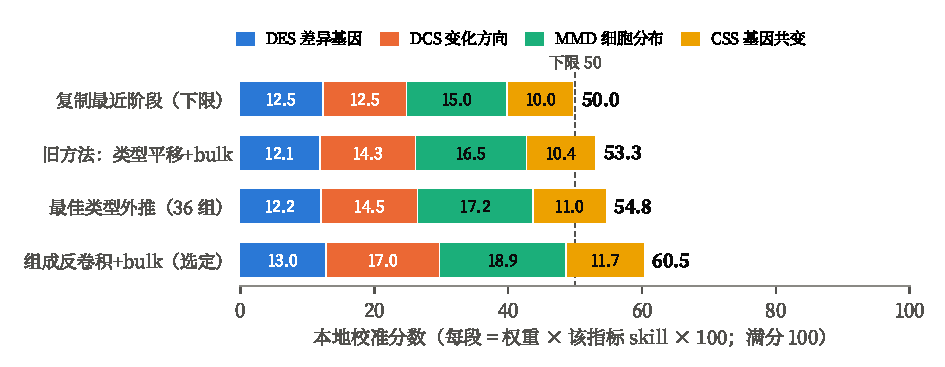
\includegraphics[width=\linewidth]{figures/fig_contributions.pdf}
\caption{第二轮选模集上的分数构成。每段为该指标的权重乘以 skill 再乘 100，四段之和为总分；复制基线每项 skill 为 0.5。四个模型使用同一组参考细胞和评价细胞。}\label{fig:contrib}
\end{figure}

图~\ref{fig:sens}a 给出了组成趋势强度 $s$ 的影响（混合比例 $\beta=1$）。分数随 $s$ 增大而上升，在 $s=3$ 左右最高，再增大就开始回落。不加表达迁移时（蓝线），$s$ 从 0.25 增加到 3，分数从 49.46 升到 59.40，说明大部分增益来自组成调整本身。从 $\bm m^\star$ 的定义看，$s=3$ 相当于把五天的 bulk 变化放大三倍后用于一天的预测。这个倍数不能理解为发育速度：式~\eqref{eq:nnls} 中的岭惩罚会把解拉回源阶段比例，需要更强的目标信号才能让比例移动，$s$ 和岭系数共同决定最终的移动幅度。

图~\ref{fig:sens}b 显示，细胞内的表达迁移在 $b=1.5$--$3$ 时只带来约 1 分的增益，$b=10$ 时降到 53.02，$b=20$ 时降到 34.80，低于复制基线。我们的理解是，bulk 数据混合了所有细胞类型，把它直接迁移到单个细胞上，幅度一大就会产生真实数据中不存在的表达状态。

\begin{figure}[t]
\centering
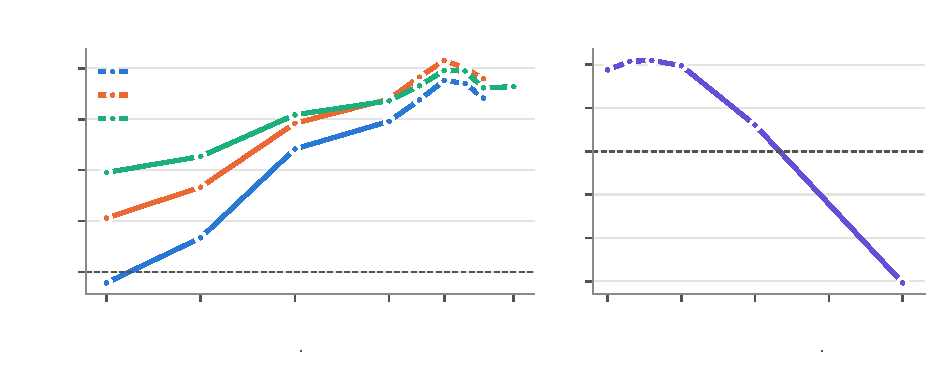
\includegraphics[width=\linewidth]{figures/fig_sensitivity.pdf}
\caption{组成反卷积的参数敏感性（选模集）。(a) 组成趋势强度 $s$，三条线对应不同的表达迁移强度，横轴为对数刻度。(b) 固定 $s=3$ 时表达迁移强度的影响；$b\le 5$ 的点来自第三批搜索（$b=5$ 为两批的平均），$b=10,20$ 来自第二批，两批抽到的源细胞不同。虚线为复制基线。}\label{fig:sens}
\end{figure}

\subsection{复核集上的回落与评价的稳定性}\label{sec:selection}

第二轮共比较了 94 条配置记录（含重复的基线），按选模集分数挑选。从多个候选中取最优，会把抽样噪声中偶然有利的部分一起选进来，选中模型在新数据上的表现通常会回落\cite{cawley}。图~\ref{fig:sel} 对比了各批前三名在选模集和复核集上的分数：12 个配置全部下降，降幅为 0.44--0.94，平均 0.72。但没有参与第二轮挑选的旧方法也从 53.27 降到 52.55，降了 0.72。所以这次回落主要来自复核集本身（它的目标细胞和锚点都不同），从这组数据看不出额外的选模偏差。选定模型相对旧方法的优势在两组细胞上几乎相同：选模集上高 7.23 分，复核集上高 7.24 分。

\begin{figure}[t]
\centering
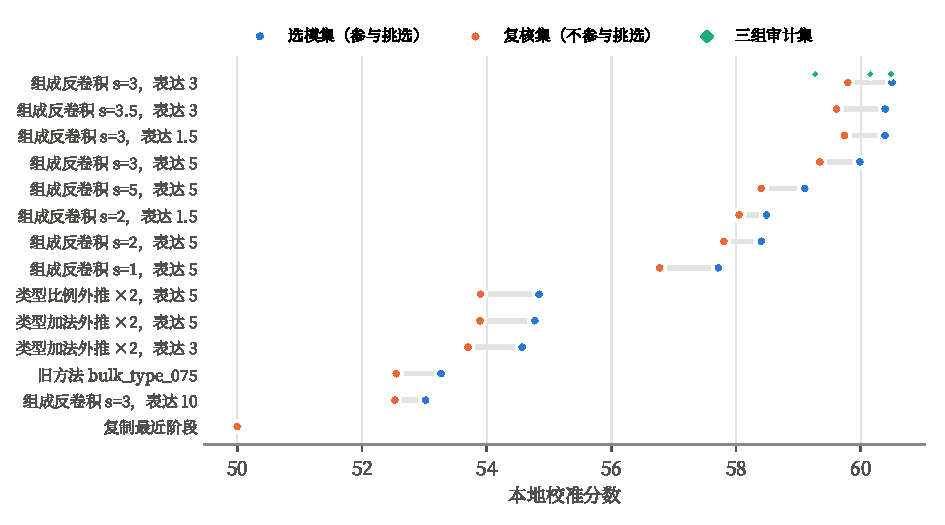
\includegraphics[width=\linewidth]{figures/fig_selection.pdf}
\caption{各批前三名、旧方法和复制基线在选模集（参与挑选）与复核集（不参与挑选）上的分数，以及选定模型在三组审计集上的分数。}\label{fig:sel}
\end{figure}

选定模型在三组审计集上得到 59.27、60.15、60.48，均值 59.97，标准差 0.63。审计时预测细胞和评分参考都固定，只换了目标细胞和上限半集，所以这个标准差只描述评价细胞抽样带来的波动（见第~3.2~节的局限）。源细胞的重新抽样也会带来波动：配置 $s=3,\beta=1,b=5$ 在两批搜索中各评了一次，因为随机数流不同，两次抽到的源细胞不同，分数分别为 59.99 和 59.80。前几名之间的差距（60.50、60.39、60.39）小于这些波动；$s$ 在 2.5--3.5、$b$ 在 1.5--3 的区域内，选模集分数最多相差 0.93，与审计标准差同一量级。所以我们只能说这个区域表现相近，不能声称某一组参数最优。

\subsection{反卷积权重不能当作生物学比例}\label{sec:weights}

表~\ref{tab:weights} 把选定模型的类型抽样权重 $\bm\pi$ 与官方公布的 E9.5 实际组成\cite{composition}放在一起。权重集中在少数类型上：横隔（ST）从 5.2\% 升到 42.4\%，房室管心肌细胞（AVC-CM）从 1.9\% 升到 17.9\%，心内膜从 9.1\% 升到 23.8\%；流出道/右心室心肌（OFT/RV-CM）、静脉窦心肌（SV-CM）等 14 个类型的权重为 0，心室心肌（V-CM）只剩 0.6\%。无放回抽样受各类细胞数限制，实际抽出的细胞组成会比权重平缓一些，但仍集中在这几个类型上。这样的组成变化很难用一天之内的发育来解释。

\begin{table}[t]
\centering\smalltable
\caption{选定模型的类型抽样权重与 E9.5 实际组成（\%）。列出全部 7 个权重不为 0 的类型，以及 E9.5 中占比较高、权重为 0 的两个类型。}\label{tab:weights}
\begin{tabular}{@{}lrr@{\hspace{2.2em}}lrr@{}}
\toprule
类型 & E9.5 实际 & 模型权重 & 类型 & E9.5 实际 & 模型权重\\
\midrule
ST（横隔） & 5.15 & 42.39 & Blood & 1.25 & 5.40\\
Endocardium & 9.12 & 23.76 & Hepatocyte & 6.98 & 1.37\\
AVC-CM & 1.91 & 17.90 & V-CM & 6.71 & 0.61\\
Epithelium & 1.37 & 8.58 & OFT/RV-CM & 10.73 & 0\\
 & & & SV-CM & 7.46 & 0\\
\bottomrule
\end{tabular}
\end{table}

我们对此的理解是：式~\eqref{eq:nnls} 拟合的是伪 bulk，只要求加权后的平均表达向目标移动；非负最小二乘的解往往是稀疏的，会选出少数几个最能把伪 bulk 推向 bulk 趋势方向的类型，DCS 和 MMD 因此改善，但这不说明 E10.5 的组成就是这样。另一种可能是 E10.5 的解剖范围包含了更多横隔等非心脏组织，按 E10.5 分数挑参数时恰好选中了拟合取样变化的组合。要区分这两种解释，需要用 E10.5 的真实组成做对照，见下一节。

\subsection{组成与表达的已知真值分析}\label{sec:oracle}

为了回答第~1~节的问题，我们设计了一组只用于分析的已知真值（oracle）条件：每个条件都让模型知道 E10.5 的一部分真实信息，用来估计各成分大致能带来多少收益。真值取自 E10.5 中不属于选模集、复核集及其上限半集的 4,000 个细胞（可能与审计集重叠），不会直接复制被评分的细胞。条件如下：
\begin{enumerate}[label=(\arabic*)]
  \item \textbf{真实全局均值}：复制基线加上真实的全局均值变化。
  \item \textbf{真实类型比例}：把 E9.5 细胞按 E10.5 的真实类型比例重抽样；标签先去掉编号后缀（如 Endocardium-1 记为 Endocardium）。
  \item \textbf{真实细胞状态}：在 2,000 个高变基因的联合 PCA 空间里为每个 E10.5 细胞找最近的 E9.5 细胞，按被选中的次数重抽样，作为“只重加权 E9.5 细胞”能达到的近似参照。
  \item \textbf{真实比例加真实类型均值}：在 (2) 的基础上，再给每个类型加上真实的均值变化。
\end{enumerate}
另外统计 E10.5 中有多大比例的细胞属于 E9.5 没有的类型（去掉编号后缀后），这部分无法靠重抽样 E9.5 细胞得到。

\pending{运行 \path{python -m experiments.oracle_decomposition --with-confirmation}，在此放表：各条件的总分和四项原始指标；E10.5 中 E9.5 不存在类型的占比；并把 (2) 的真实比例与表~\ref{tab:weights} 的模型权重对比，判断第~\ref{sec:weights}~节的两种解释哪个成立}

\subsection{隐藏测试集结果}\label{sec:test}

两次正式提交的官方分数见表~\ref{tab:test}。测试榜的评分参考是最后一个训练阶段 E9.5，和本地评价相同。作为参照，表中还列出公开测试榜上方法名写着用真实细胞（real cells 或 real nuclei）的三个条目和榜首。这三个条目只有一个写明是 E10.5 的细胞，做法都没有公开，名字里还有 extrapolation、maturity tilt、coarse-type 等字样，看来也对真实细胞做过处理；表中给的是三者各项的范围，不是同一个条目的分数。

\begin{table}[h]
\centering\smalltable
\caption{官方 E12.5 测试集分数（各项为技能分，复制 E9.5 参考 = 50，另一半真值 = 100）。参照行取自 2026 年 11 月 26 日 10:25 的公开测试榜\cite{leaderboard}。}\label{tab:test}
\begin{tabularx}{\linewidth}{@{}Yrrrrr@{}}
\toprule
提交 & 总分 & DES & DCS & MMD & CSS\\
\midrule
第一次：保守版 h1（第二轮组成反卷积） & 70.62 & 66.3 & 76.9 & 69.0 & 70.5\\
第二次：第九轮文件（第~\ref{sec:negative}~节） & 73.37 & 65.8 & 82.3 & 72.4 & 73.0\\
\midrule
参照：方法名写着用真实细胞的三个条目 & 77.07--80.57 & 71.4--73.2 & 79.9--83.6 & 75.0--87.4 & 77.0--78.0\\
参照：榜首 & 86.32 & 81.9 & 89.7 & 86.4 & 87.6\\
\bottomrule
\end{tabularx}
\end{table}

第二次比第一次高 2.75 分，增益来自 DCS、MMD 和 CSS，DES 略降；它在 554 支队伍中排第 352 名。两次提交都低于这三个参照条目，第二次比它们低 3.7--7.2 分，差在 DES、MMD 和 CSS 三项，DCS 与它们相当。第一次提交有一半细胞来自测得很浅的第 1、2 个文库，这也会拉低分数。本地选模集上的 60.50 分和这里的分数参考阶段相同，但真值和抽样不同，不能直接比较。

\subsection{第二次提交：一个反面案例}\label{sec:negative}

第二次提交的文件有 5,000 个细胞，由 E10.5 第 3 个测序文库（细胞条码后缀 \_3）的 4,997 个不同的真实细胞改出来。这个文库 94\% 是心脏或血细胞类型，测序深度接近 E8.5、E9.5 的文库。改动依次是：
\begin{enumerate}[label=(\arabic*)]
  \item 每个细胞先随机保留约 85\% 的分子（二项抽样）；
  \item 55\% 的细胞按文库原有的类型组成抽取，另外 45\% 按外部 E14.5 心脏样本（GEO GSM8394736\cite{gsm8394736}，单细胞核测序）的细胞类型组成抽取；
  \item 血细胞和非心脏类型以外的细胞（共 4,193 个），在本类型 E10.5 几乎不表达的基因上（类型均值低于每万计数 0.3），自己的分子保留 75\%，再按同类型一个 E14.5 细胞核与其 19 个近邻的合并表达补入 25\%，别的谱系的标志基因不补；
  \item 两项发育位移：心肌、心内膜和心外膜细胞中，只有从 E9.5 到 E10.5 已经朝同一方向变化的基因才向 E14.5 的水平移动；全部细胞再按外部 bulk 趋势（GSE223237\cite{gse223237}，第~2.2~节）移动两天的量。
\end{enumerate}
这套方法经过第四到九轮迭代，各步的取舍依据是本地代理（E8.5、E9.5 到 E10.5）、在 E10.5 细胞上模拟的若干种“假设的 E12.5”，以及第一次提交的四项分数。

第 (2)--(4) 步共同依据一个判断：E12.5 的组成和表达已经从 E10.5 向 E14.5 走了一半左右。这个判断主要来自第一次提交的分数。我们在本地构造了一系列假设的 E12.5，计算第一次提交在每种假设下应得的四项分数；与实际分数最接近的是“心脏文库细胞加 30\%--60\% 的 E14.5 细胞核”这一类假设，三档之间分不太开，文件取 45\%。测试结果说明这个判断很可能高估了 E12.5 与 E10.5 的差别：第二次提交比参照条目低在 DES、MMD 和 CSS，其中 MMD（72.4 对 75.0--87.4）直接受细胞组成影响。这是推断，只凭一次提交的四项分，无法拆出每一步各丢了多少。

这一推断有三处弱点。第一，这种吻合度衡量的是假设离第一次提交有多远。我们在“细胞表达向 E14.5 挪多少”这一维上发现它分不清方向，因此弃用了那一维；在组成比例上，它在两个答案已知的情形里选对了方向，所以留用。后来发现它在另一个参数（第 (3) 步的混合比例）上同样偏向离第一次提交更远的假设，组成比例上是否也有这个偏向没有再查。第二，这一类假设预告第一次提交的 CSS 为 0.56--0.62，实际是 0.705；第 (1) 步正是为了解释这一项而加的，它本身也可能丢分。第三，本地有一项“零时间差”检验，假设 E12.5 与 E10.5 心脏文库完全相同，用来衡量每一步改动的代价：原样的心脏文库在这项检验中得 99.8 分，第七、八轮的配方约 83 分。确定组成比例时，这项检验的权重被压得很低，理由是第一次提交的分数说明 E12.5 离 E10.5 心脏文库很远，以及发育隔了两天；后来它被提到和其他检验同等的权重，但只用来拦新增的改动，已有的组成改动没有按它重新评价。第二次提交低于参照条目，和这项检验的提示不矛盾；不过原样的心脏文库在测试上能得多少并不知道。

这个案例给出三点教训。其一，本地代理能检验一种做法在已知的一步变化上是否有效，检验不了目标阶段具体是什么样子；改动越依赖后者，本地分数越不可信。其二，只有一次真实反馈时，用它反推目标的性质很不可靠，能吻合的假设太多，在一些参数上还会偏向离反馈更远的假设。其三，两次提交机会中最好有一次交最简单的版本（例如 E10.5 心脏文库原样），作为另一次的参照；这次两次提交都改动了细胞组成，没有和“不改动”直接比较的机会。第二轮的本地实验中，组成调整带来了主要增益（表~\ref{tab:main}），两次正式提交却都在 MMD 上偏低，我们推测 E9.5 到 E10.5 这一步的经验不一定适用于 E12.5。

第二次提交的方法说明披露了上述做法、全部外部数据、AI 编码助手的参与、第一次提交的返回分数的四处用途（选择 E14.5 组成的比例；检查第 (4) 步第一项位移；定性地决定零时间差检验的权重；选择第 (1) 步保留的分子比例），以及参考过公开测试榜。竞赛规则允许用返回的分数在已经做好的预测之间选择，禁止从分数中反解目标的性质再用来构造预测\cite{rules}。我们用第一次提交的分数推断 E12.5 的细胞组成走了多远，再按推断出的 45\% 定文件，第二批候选的范围也是看过第一批的吻合程度后才定的，这和规则禁止的做法很接近。各轮的代码、评分表、运行记录和说明见 \path{experiments/round4_direction.py} 和 \path{experiments/round5_seed42/} 至 \path{experiments/round9_seed42/}，复盘全文见 \path{reports/final/T1_第二次提交复盘.md}。

\section{困难、解决办法与局限}

表~\ref{tab:issues} 列出了研究过程中遇到的主要问题和我们的处理方式。

\begin{table}[h]
\centering\smalltable
\caption{主要困难与处理}\label{tab:issues}
\begin{tabularx}{\linewidth}{@{}p{3.6cm}Y@{}}
\toprule
困难 & 处理方式与效果\\
\midrule
复制基线不是 50 分 & 早期实验中预测细胞与评分参考分别抽样，复制基线只得 45.86。改为对齐参考后，模型之间可以公平比较（第~\ref{sec:linear}~节）。\\
加性平移破坏零值结构 & 非零比例从 12\% 升到 27\%--50\%，CSS 变差。改用保零平移后 CSS 恢复到基线水平。\\
注释词表不统一 & 相邻阶段同名类型只占约一半，且有拆分（Endocardium-1/2）。类型条件模型只用两阶段都有的类型；已知真值分析中去掉编号后缀再匹配。\\
时间点太少 & 两个训练阶段只能估计一个变化方向。引入合规的外部 bulk 数据，用跨重复一致性和表达量收缩估计基因趋势。\\
选模偏差 & 选模集与复核集分开，复核集只评不选，再用三组审计集检查；同时用未参与挑选的旧方法作参照，区分选模偏差和评价集本身的差异。\\
大矩阵的内存 & 单个阶段的文件约 600 MB，E9.5 全部细胞转成稠密矩阵超过 2 GB。按行分块读取 AnnData，只把抽出的子样本转成稠密矩阵。\\
\bottomrule
\end{tabularx}
\end{table}

仍然存在的局限有以下几点。
\begin{itemize}
  \item \textbf{本地验证不能检验两天外推}：所有选择都基于 $h=1$ 的预测。E10.5 到 E12.5 跨两天，E9.5 到 E10.5 时约一半细胞所属的类型在前一阶段没有同名对应，E12.5 很可能也有新出现的类型，隐藏测试的分数可能比本地分数低。h1 与 h2 哪个更好，本地数据无法判断。
  \item \textbf{评价集共用一个样本}：第~\ref{sec:selection}~节的波动只反映细胞抽样；结论能否推广到其他胚胎，还取决于胚胎间的差异，而每个阶段只有一个样本。
  \item \textbf{组成权重缺乏生物学解释}：第~\ref{sec:weights}~节显示权重集中在少数类型上，模型的改进可能部分来自拟合取样范围的变化。
  \item \textbf{DES 几乎没有提高}：所有方法的 DES 都在 0 附近或为负，选定模型在复核集上也只有 0.036。可能的原因是 bulk 趋势混合了所有细胞类型，又来自另一项研究的样本，按它排出的差异基因只比按表达量排序略好。
  \item \textbf{自动化搜索}：第二轮的配置由代码助手协助设计并逐批运行（见 AI Assistance Statement），后续批次的范围依据前批的选模集分数确定。这仍是在选模集上的反复搜索，所以我们用复核集和审计集检查结果，并在第~\ref{sec:selection}~节报告了回落。
\end{itemize}

\section{结论}

在只有两个训练阶段的条件下，直接平移表达均值的外推方法没有超过复制基线；按指标拆分，原因是按均值差排出的差异基因不如按表达量排序（DES 为负），以及加性平移改变了零值结构（CSS 变差）。引入外部 bulk 趋势并据此调整细胞类型比例后，本地分数从 50 提高到约 60，增益主要来自变化方向和细胞状态分布两项指标，而只改变表达水平的模型在细胞状态分布上增益很小。这支持“组成变化在本任务中很重要”的判断。同时，这一改进依赖于一组集中、难以解释的类型权重，模型给出的具体比例还不能作为生物学结论。两次官方提交（70.62 和 73.37 分）都低于公开榜上方法名写着用真实细胞的条目。第二次提交的复盘（第~\ref{sec:negative}~节）表明，凭第一次提交的分数推断 E12.5 的组成、再据此改动细胞，很可能是它丢分的主要原因，但只凭四项分无法确认。\pending{已知真值分析的结果出来后，在此补一句：组成与表达各自能解释多少差距}

\section*{成员贡献}

\pending{按实际分工填写，每人一两句，写清具体做了哪些部分。开题时的分工为：高景行负责数据获取、预处理与基本数据分析；王恒毅负责团队注册、参考基线、预测文件生成与官方提交；李凯瑞负责低维外推、分层扩展与消融实验；崔帅达负责评价代码与误差解释。}

\section*{Code and Data Availability Statement}

代码、配置、逐次实验的评分表和运行记录公开在 \url{https://github.com/ManchesterCityWhy/Statistical_Learning_Term_Project}。\path{t1_pipeline/README.md} 说明环境安装、官方基因列表的下载和数据放置位置；\path{experiments/README.md} 与 \path{experiments/round2_seed42/README.md} 列出复现每轮实验的命令；本报告的三张图可由 \path{python reports/final/make_figures.py} 从仓库中的评分表重新生成。依赖版本见 \path{t1_pipeline/requirements.txt}（第一轮）和 \path{experiments/round2_seed42/requirements.txt}（第二轮），评价指标使用 veckit 的固定提交 \texttt{cc3859ab}。所有随机过程的种子写在脚本和配置中（第二轮为 42，第一轮为 0、31、101 或 7、19、42）。

竞赛数据需在 Virtual Embryo Challenge 注册后下载\cite{data}，E10.5 验证数据需在决赛阶段申请，按数据条款不在仓库中重新分发；训练文件的 SHA-256 写在代码中，用于核对版本。外部数据均可从 GEO 公开下载，所用样本编号见第~2.2~节，文件校验值记录在各次运行的 manifest 中。预测文件不放入仓库，第一次提交的校验值见 \path{experiments/round2_seed42/prediction_h*_manifest.json}，第二次提交的见 \path{experiments/round9_seed42/manifest.json}。第四到九轮另用了外部 E14.5 心脏单细胞核数据 GSM8394736（GEO GSE272154），它和 bulk 数据一样在规则允许的时间窗口之外，文件校验值也记录在 manifest 中。

\section*{AI Assistance Statement}

本项目使用了以下 AI 工具：
\begin{itemize}
  \item \textbf{ChatGPT}：开题阶段用于讨论想法和润色部分文字。
  \item \textbf{OpenAI Codex}：用于实现第一、二轮的数据检查、评价和预测代码，下载与校验外部数据，协助设计第二轮的候选搜索并逐批运行，以及整理实验记录。
  \item \textbf{Claude（Anthropic，通过 Claude Code 使用）}：用于审阅评价设计，编写熵平衡与已知真值分析两个脚本及其测试，从仓库中的评分表生成本报告的图，以及起草本报告和汇报幻灯片。第四到九轮（2026 年 11 月 25 日晚至 26 日）的方法、实验、选模规则、第二次正式提交的预测文件和方法说明、提交前的分数估计，都由 Claude Code 设计、实现和运行；第~\ref{sec:test}~节、第~\ref{sec:negative}~节和复盘文档也由它起草。
\end{itemize}
第一到三轮的研究问题、评价方案和选模规则由小组讨论确定；第四到九轮的选模规则由 Claude Code 在每批实验运行前写入运行记录。竞赛中我们按 Human Team 参赛：规则第 9 节规定，人阅读中间结果并据此指挥下一步的条目属于 Human Team\cite{rules}，第四到九轮是这样进行的。报告中的数字均来自仓库内的评分表和运行记录；作图所需的锚点 $m_f,m_c$ 由评分表中的分数反算，与表中分数的误差小于 $10^{-12}$。\pending{写明第四到九轮由谁指挥、在谁的计算机上运行，两次官方提交各由谁上传，以及组员如何核查 AI 生成的代码、数字和文字（谁核查了哪部分）}

\begingroup
\small
\setlength{\parskip}{0pt}
\begin{thebibliography}{99}
\setlength{\itemsep}{2pt}
\bibitem{schiebinger}
Schiebinger G, Shu J, Tabaka M, et al. Optimal-transport analysis of single-cell gene expression identifies developmental trajectories in reprogramming. \textit{Cell}, 2019, 176(4): 928--943.
\bibitem{task}
Virtual Embryo Challenge. Task 1: Temporal. \url{https://virtualembryo.ai/challenge/tasks/temporal}.
\bibitem{data}
Virtual Embryo Challenge. Data. \url{https://virtualembryo.ai/challenge/data}.
\bibitem{rules}
Virtual Embryo Challenge. Official Rules. \url{https://virtualembryo.ai/challenge/rules}.
\bibitem{gse223237}
NCBI Gene Expression Omnibus. GSE223237. \url{https://www.ncbi.nlm.nih.gov/geo/query/acc.cgi?acc=GSE223237}.
\bibitem{gsm6211349}
NCBI Gene Expression Omnibus. GSM6211349. \url{https://www.ncbi.nlm.nih.gov/geo/query/acc.cgi?acc=GSM6211349}.
\bibitem{gsm8394736}
NCBI Gene Expression Omnibus. GSM8394736（GSE272154，RNA Wild Type e14.5 rep1）. \url{https://www.ncbi.nlm.nih.gov/geo/query/acc.cgi?acc=GSM8394736}.
\bibitem{perinatal}
CZ CELLxGENE Discover. Mouse perinatal heart maturation scRNA-seq（原始数据 GEO GSE109247、GSE150817；\textit{Biology Open}, doi:10.1242/bio.062493）. \url{https://cellxgene.cziscience.com/collections/613f5480-4957-4f80-b804-0e2b85ac454c}.
\bibitem{evaluation}
Virtual Embryo Challenge. Evaluation: Task 1 scoring. \url{https://virtualembryo.ai/challenge/evaluation?section=scoring&task=1}.
\bibitem{bh}
Benjamini Y, Hochberg Y. Controlling the false discovery rate: a practical and powerful approach to multiple testing. \textit{Journal of the Royal Statistical Society, Series B}, 1995, 57(1): 289--300.
\bibitem{gretton}
Gretton A, Borgwardt K M, Rasch M J, et al. A kernel two-sample test. \textit{Journal of Machine Learning Research}, 2012, 13: 723--773.
\bibitem{scheuerer}
Scheuerer M, Hamill T M. Variogram-based proper scoring rules for probabilistic forecasts of multivariate quantities. \textit{Monthly Weather Review}, 2015, 143(4): 1321--1334.
\bibitem{veckit}
aristoteleo/veckit, commit cc3859ab2a2305efc4544815d3f44f660efa77d4. \url{https://github.com/aristoteleo/veckit}.
\bibitem{nnls}
Lawson C L, Hanson R J. \textit{Solving Least Squares Problems}. Englewood Cliffs: Prentice-Hall, 1974.
\bibitem{deville}
Deville J C, S\"arndal C E. Calibration estimators in survey sampling. \textit{Journal of the American Statistical Association}, 1992, 87(418): 376--382.
\bibitem{hainmueller}
Hainmueller J. Entropy balancing for causal effects: a multivariate reweighting method to produce balanced samples in observational studies. \textit{Political Analysis}, 2012, 20(1): 25--46.
\bibitem{efraimidis}
Efraimidis P S, Spirakis P G. Weighted random sampling with a reservoir. \textit{Information Processing Letters}, 2006, 97(5): 181--185.
\bibitem{leaderboard}
Virtual Embryo Challenge. Leaderboard, Task 1（测试榜与冻结验证榜，2026-11-25、11-26 访问）. \url{https://virtualembryo.ai/challenge/leaderboard}.
\bibitem{cawley}
Cawley G C, Talbot N L C. On over-fitting in model selection and subsequent selection bias in performance evaluation. \textit{Journal of Machine Learning Research}, 2010, 11: 2079--2107.
\bibitem{composition}
Virtual Embryo Challenge. Task 1 released-stage composition. \url{https://virtualembryo.ai/challenge/panels/t1_composition.json}.
\end{thebibliography}
\endgroup
\end{document}
